\documentclass[12pt]{article}

\usepackage{amsmath}
\usepackage{amssymb}
\usepackage{amsthm}

\usepackage{geometry}

\usepackage{tikz}
\usetikzlibrary{arrows}

\title{CS420 - Homework \#1}
\author{Trevor Bramwell}
\date{\today}

\begin{document}
\maketitle

\section*{Problem 1}

Throughout the lecture, we assumed that no two edges in the input graph
have equal weights, which implies that the minimum spanning tree is
unique. In fact, a weaker condition on the edge weights implies MST
uniqueness.

\subsection*{(a)}
Describe an edge-weighted graph that has a unique minimum spanning tree,
even though two edges have equal weights.

\begin{center}
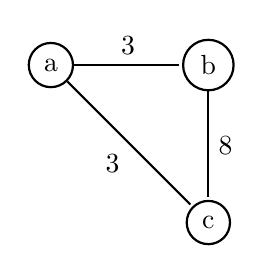
\begin{tikzpicture}[-,>=stealth',shorten >=1pt,auto,node distance=2cm,
                    thick]
  \tikzstyle{every state}=[fill=white]

  \node[draw, circle]   (A)              {a};
  \node[draw, circle]   (B) [right of=A] {b};
  \node[draw, circle]   (C) [below of=B] {c};

  \path (A) edge node {$3$} (B)
            edge [below left] node {$3$} (C)
        (B) edge node {$8$} (C);
\end{tikzpicture}
\end{center}

\subsection*{(b)}
Prove that an edge-weighted graph $G$ has a unique minimum spanning tree
if the following condition holds:

\begin{itemize}
    \item For any partition of the vertices of $G$ into two subsets, the
          minimum-weight edge with one endpoint in each subset is unique.
\end{itemize}

\begin{proof}[Proof by Contradiction]
    Let $G$ be an edge-weighted graph. Let $T_1$, $T_2$ be arbitrary
    partitions of $G$.
    
    Assume the minimum-weight edge with one endpoint in each subset is
    not unique.

    Then $\exists$ some edges $e_1$ and $e_2$ which have one endpoint in each
    subset.

    $\ldots$

\end{proof}

\subsection*{(c)}
Describe and analyze an algorithm to determine whether or not a graph
has a unique minimum spanning tree.

\end{document}
